\chapter{Methods for studying environmental noise}

Environmental noise refers to any signal originating from outside the structure of a \ac{GW} detector that can impact the detector's sensitivity or disrupt its ability to achieve and maintain lock~\citep{Effler_2015,Nguyen_2021}.
The effects of environmental noise on detector sensitivity can range from persistent excess noise in the \ac{GW} strain data, to short-duration transient signals, or \textit{glitches}.

One goal of studying environmental noise is to aid in the validation of \ac{GW} events.
Due to the sophisticated nature of the search pipelines used to detect gravitational waves in the \ac{LIGO} data, environmental glitches are highly unlikely to fully account for a \ac{GW} event candidate.
That said, glitches capable of influencing analyses occur frequently at both observatories.

Unlike instrumental noise, environmental noise can potentially be correlated between different detectors, i.e. stemming from a common source as opposed to stemming from chance coincidence.
Such correlated noise is not accounted for in the estimation of false-alarm probabilities, which is done by time-shifting background data from each \ac{LIGO} detector to produce long stretches of coincident background.

Environmental noise is particularly important in searches for un-modeled sources of gravitational waves, as these look for excess power without the use of waveform templates.
Even for highly significant \ac{CBC} events, contamination of the strain data can be detrimental to parameter estimation analyses that infer source properties from the morphology of the event.
Thus it is important to have a quantitative solution for identifying and evaluating the impact of environmental transients when they occur coincide with candidate events.

The second goal is to improve the sensitivity and performance of the detector by localizing noise sources and coupling mechanisms. Once tracked down, they can be mitigated by eliminating the noise sources, attenuating the propagation of the signal, or modifying the detector itself.

In this chapter I introduce sources of environmental noise (Section~\ref{sec:noise-sources}), describe the hardware used to monitor those noise sources (Section~\ref{sec:pem-channels}) and to reproduce them experimentally (Section~\ref{sec:injections}).
I present a method for quantifying environmental coupling (Section~\ref{sec:cf}), then I discuss the limitations (Section~\ref{sec:uncertainties}) and software implementation (Section~\ref{sec:pemcoupling}) of the method.

\section{Sources of environmental noise}\label{sec:noise-sources}

The environment can influence a \ac{GW} detector through physical contact (via vibrations or temperature fluctuations), electromagnetic waves, static electric and magnetic fields, and possibly high-energy radiation.

Vibrations can affect the data by directly moving the test masses.
They can also modulate the paths of light that is scattered off of surfaces inside the interferometer, or introduce fluctuations in the alignment of the input laser beam.

\section{The PEM sensor array}\label{sec:pem-channels}

\begin{figure}[h!]
	\centering
	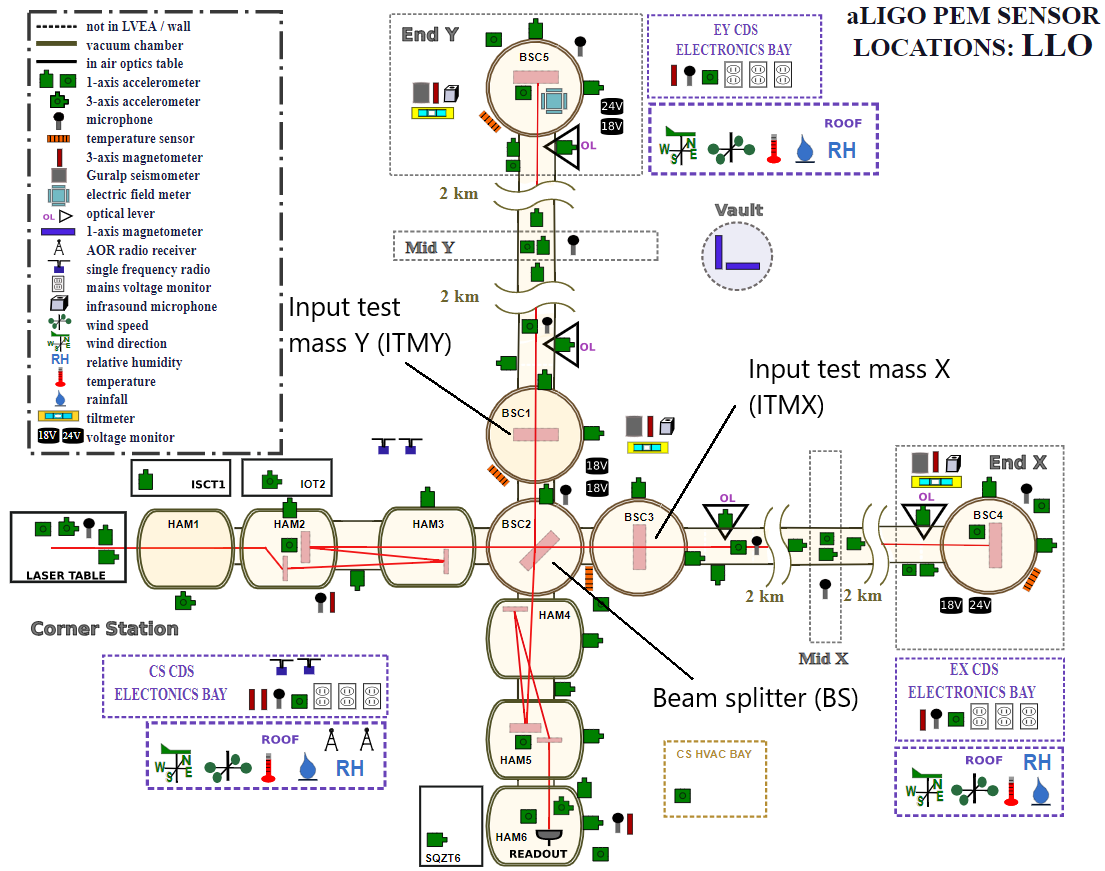
\includegraphics[width=\textwidth]{figures/noise-methods/pem-channels.png}
	\caption{\raggedright The PEM system layout at LLO during O3, as seen on the PEM public website.}
	\label{fig:pem-channels}
\end{figure}

Understanding environmental influences on the detectors requires comprehensive monitoring of its physical surroundings.
This is done through the \ac{PEM} system of auxiliary sensors (Figure~\ref{fig:pem-channels}), which consists of accelerometers for high-frequency vibrations (between tens to thousands of Hertz), seismometers for low-frequency vibrations (up to tens of Hertz), microphones, magnetometers, voltage monitors that measure the voltage of electric power supplied to the detector sites, radio-frequency (RF) receivers, a cosmic-ray detector for high-energy particles, and wind, temperature and humidity sensors.
Detailed information on \ac{PEM} sensors, including example background spectra and calibration data, can be found on the \ac{PEM} website, PEM.LIGO.org~\citep{PEM_website}.

Most sensors produce an analog signal that is converted to a digital signal via an \ac{ADC}, then processed by a data acquisition system and saved into frame files.
The frame file are the primary data format for \ac{GW} detector data~\citep{frame_file} and are remotely accessible via the \ac{LIGO} grid computing clusters located at the observatories as well as various \ac{LIGO}-affiliated institutions.
From here on, I will use \textit{sensor} to refer to the physical monitoring device and \textit{channel} to refer to the data stream as read from frame files.

\subsection{Monitoring the monitors with \ligocam}\label{sec:ligocam}

Maintaining an extensive, ever-expanding array of auxiliary sensors requires a scalable solution for monitoring their behavior.
Frequent changes to the sensors, as well as of interferometer hardware, result in changes in ambient spectral characteristics.
Worse yet, sensors, their power supplies, their \acp{ADC}, and the data acquisition system that process their signals all have the potential to malfunction, leaving blind spots in our ability to detect signals that may affect the \ac{GW} strain data.

The \ac{LIGO} channel activity monitor, or \ligocam, is a program that checks for various signs of unusual sensor behavior using a number of spectral cues~\citep{ligocam}.
The goal of \ligocam is to produce human-readable summaries of sensor behavior for the entire \ac{PEM} network at an observatory, and send email alerts to experts when significant malfunctions are identified.

Leveraging the \ac{LIGO} data grid computing clusters, \ligocam parallelizes its analysis by splitting the full channel list (over 100 channels), processing only five per job.
This allows it to run hourly, scheduled by a \code{cron} job, outputing a summary page and transmitting email alerts (if applicable) within minutes.
A \code{cron} job is scheduled at each of the \ac{LIGO} observatories.
Although such expediency is not necessary for fixing malfunctioning hardware, it is important to have up-to-date channel status when validating recently detected \ac{GW} event candidates, as discussed in Section~\ref{sec:vetting}.

The program reads in time series data using the \code{gwpy} library~\citep{gwpy} and converts each time series to an \ac{ASD}.
When run for the first time, \ligocam saves the current \acp{ASD} as reference \acp{ASD}.
On each subsequent run at a later time $t$, the new \ac{ASD} $X_t(f)$ is compared to the reference $\overline{X}_{t-1}(f)$ to determine if there is anomalous behavior present.
If $X_t(f)$, shows no anomalous behavior relative to $\overline{X}_{t-1}(f)$, then the reference is updated as an exponential average of all past non-anomalous \acp{ASD}:

\begin{equation}
	\overline{X}_t(f) =
		\begin{cases}
			X_0(f), & t=0\\
			\alpha X_t(t) + (1 - \alpha) \cdot \overline{X}_{t-1}(f), & t > 0
		\end{cases}
\end{equation}
where $\alpha^{-1}$ is the averaging decay length.
If \ligocam is run hourly with $\alpha^{-1}=1/6$, for instance, then $\overline{X}_t(f)$ is roughly the average of the past six hours of channel data.
If any anomalous behavior is detected, it is reported on the output HTML page and (if sufficiently egregious) via email to the relevant parties, and $\overline{X}_t(f)$ is not updated.

Anomalies are identified and reported in a number of ways.
Noise far above or below the reference is a sign of changes to hardware or infrastructure in the vicinity of the sensor, which may not adversely affect coverage of the area but could adversely affect nosie estimates as described in Section~\ref{sec:vetting}.
If $X_t(f)$ is many orders of magnitude below the reference but still above the electronic noise background of the \ac{ADC}, the sensor is considered to be faulty.
Some sensors, especially magnetometers, can have background noise levels low enough to be near the \ac{ADC} noise floor.
For this reason, checks for magnetometers are performed specifically on the 60\,Hz mains signal, while other sensors (accelerometers, microphones, etc.) are analyzed for broadband variations.
If the signal is even weaker than the electronic noise background, then the data acquisition system is blamed for the failure.

\section{Environmental noise injections}\label{sec:injections}

\begin{figure}[h!]
	\centering
	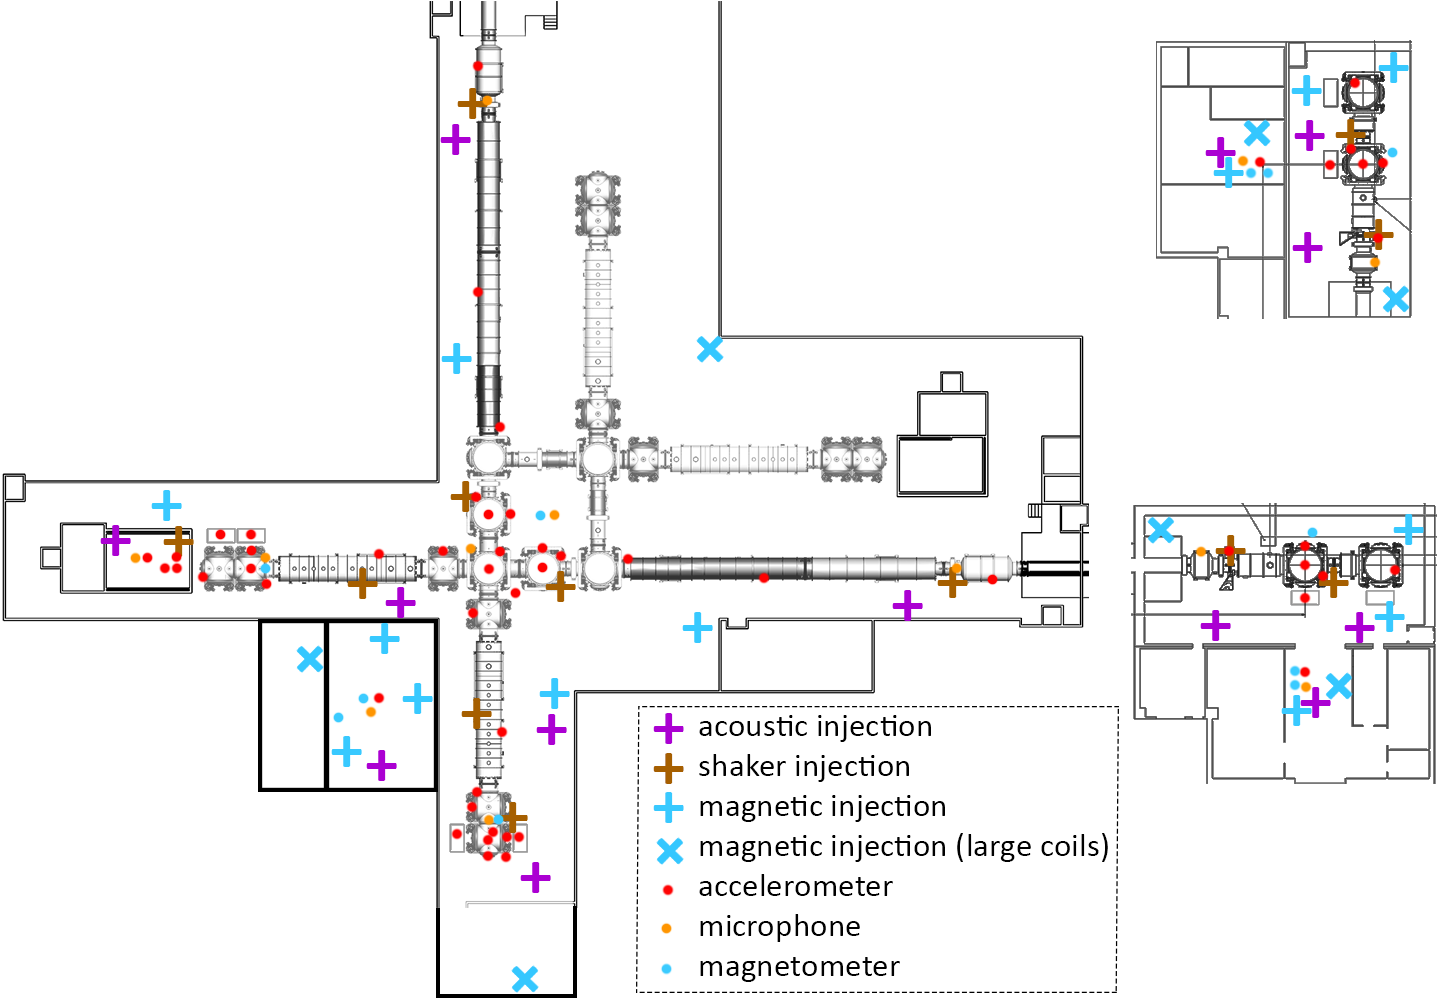
\includegraphics[width=\textwidth]{figures/noise-methods/injection-map.png}
	\caption{\raggedright
		Standard locations for vibration and magnetic injections at the LHO corner station (left), Y end station (top right), and X end stations (bottom right).}
	\label{fig:injection-map}
\end{figure}

The effect of environmental influences on the sensitivity of a \ac{GW} detector can be studied by making noise \textit{injections}.
These are signals produced by human-operated sources with the intention of replicating environmental disturbances with sufficient amplitude to produce excess noise in the \ac{DARM} spectrum.
The amplitude of the excess, combined with measurements of the input signal, can be used to quantify the coupling behavior (Section~\ref{sec:cf}).
The most common examples are acoustic injections, generated using speakers, seismic injections generated by vibrational shakers, and magnetic field injections generated by electrical current loops.

At each observatory we inject from 13 locations with acoustic injections, about 12 with shaking injections, and 15 with small-coil magnetic injections, with 7 large-coil magnetic injection locations planned for \ac{O4} (as explained in Section~\ref{sec:injections-magnetic}).
The number and locations of shaker injections vary between injection campaigns. For all injection types, multiple injections are made at each location in order to focus on different frequency bands.
Additionally, impulse injections (not shown) are made at locations where vibrational injections have revealed strong coupling sites.

\begin{table}[h!]
	\centering%
	\caption{\label{tab:injectors}Specifications for injection equipment.}
	\begin{tabularx}{\linewidth}{X>{\hsize=.3\hsize}X}
		\toprule
		Equipment & Injection type \\
		\midrule
		Custom enclosure with two 14-in. speakers & Acoustic\\
		Various smaller speakers & Acoustic\\
		APS 113 Electro-Seis\reg Long Stroke Shaker~\citep{big_shaker} & Vibrational\\
		Piezosystem\reg~\citep{piezo} shaker with custom reaction mass & Vibrational\\
		Br\"uel \& Kj\ae r\reg~\citep{bk} EM shaker with custom reaction mass & Vibrational\\
		1\,m diameter copper coil (100\,turns) & Magnetic\\
		3\,x\,3\,m and 5\,x\,5\,m coils (80-100\,turns) & Magnetic\\
		\bottomrule
	\end{tabularx}
\end{table}


Injection locations are chosen to best mimic disturbances from outside the detector (Figure~\ref{fig:injection-map}).
To do so we choose them to be as far from the detector and environmental sensors as possible, but we are usually limited by the size of the detector sites themselves (some injections can be made from outside).
Time dedicated to these tests has to be balanced against other instrumental work and observing time, which leads to a trade-off between measurement uncertainty and coverage.
We perform injections from as many locations as time allows in order to maximize coverage of potential coupling sites.
Increased time allocation toward environmental studies in recent years has allowed for a significant increase in the number of injection locations.
Table~\ref{tab:injectors} summarizes the current equipment used and Figure~\ref{fig:injection-equipment} shows photos of some of the equipment.

\begin{figure}[h!]
	\centering
	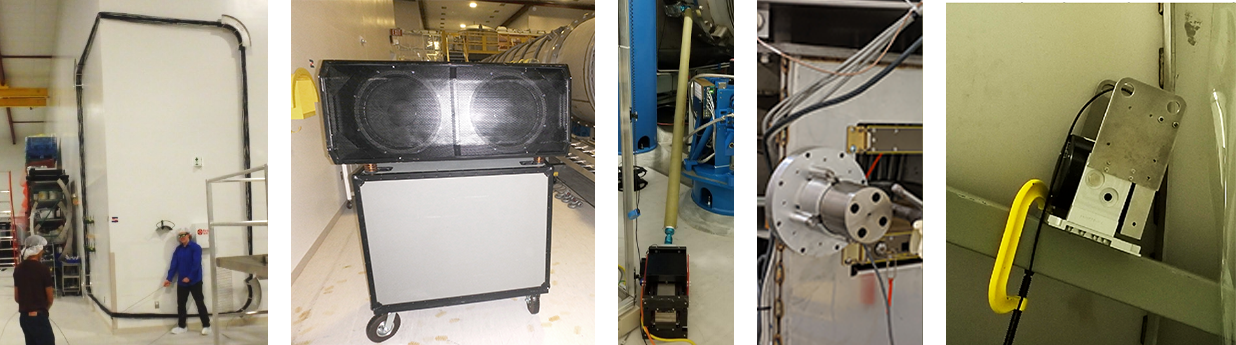
\includegraphics[width=\textwidth]{figures/noise-methods/injection-equipment.png}
	\caption
	[Injection equipment photos]
	{\raggedright
	Injection equipment photos. From left to right: wall-mounted magnetic field injection coil; 14-in. speakers; APS 113 shaker connected to the door of a vacuum chamber by a rigid fiberglass rod; modified Piezosystem shaker clamped to an electronics rack; modified B\&K shaker clamped to a beam tube support.}
	\label{fig:injection-equipment}
\end{figure}

\subsection{Vibrational injections}~\label{sec:injections-vib}

Acoustic injections are produced by large speakers.
For the corner stations, a pair of speakers mounted on a vibrationally isolated cart (to minimize ground-based vibrational signals) are used.
Typically, the injection signal is white noise band-passed between 20-2000\,Hz, with narrower bands being used for special follow-up of particular coupling sites.

Seismic injections at low frequency (up to tens of Hertz) during \ac{iLIGO} were performed with small electromagnetic and piezoelectric shakers and a weighted cart.
A large shaker has been used since the beginning of noise studies for \ac{O3}.
The large shaker can impart up to 133\,N of sine force and a peak-to-peak displacement of 158\,mm~\citep{big_shaker}, compared to the electromagnetic shaker which imparts up to 45\,N of force and a displacement of 8\,mm~\citep{bk}.
While smaller shakers can be directly clamped to the interferometer supports, a rigid fiberglass rod is used to connect the large shaker to the interferometer.
This has an added benefit of being better able to adjust the direction of the actuation by angling the rod and shaker accordingly.

Two new injection techniques have been developed for localizing vibration coupling sites connected to the vacuum enclosure, such as locations on the vacuum enclosure that reflect scattered light.
The techniques rely on the slow propagation speeds (hundreds of meters per second) of vibrations on the steel vacuum enclosure walls or, for acoustic injections, in air.
These two techniques were essential in the localization of coupling sites in \ac{O3}, as discussed in Section~\ref{sec:vib}.

\subsubsection{Beating-shakers technique}~\label{sec:injections-vib-beats}

The beating-shakers technique is narrow-band, and involves vibrating the vacuum enclosure at two slightly different frequencies, each injected from a shaker or a speaker at a different location (e.g. a shaker at one location injects a sine wave at frequency $f$ and a shaker at the other location injections at frequency $f + 0.01$\,Hz).
The two injections are adjusted in amplitude to produce strong beats in the \ac{GW} channel.

Because the injection locations are different, the relative phase of the two injected signals varies with location on the vacuum enclosure.
As a result, the phase of the beat envelope varies with position, and different sites experience maximum chamber wall motion at different times.
The sites with accelerometer signals that have the same beat envelope phase as the \ac{DARM} signal are candidates for the scattering sites on the vacuum enclosure walls.
Other sensors that are not near the coupling site may also match the phase by chance, but these false positives can be rejected by varying the locations of the shakers.

\subsubsection{Impulse injections}~\label{sec:injections-vib-impulse}

The second injection technique, which is broad band, involves propagation delays in impulse injections.
Impulse injections are performed by striking the vacuum enclosure directly with enough force to produce a transient in the \ac{GW} channel and in nearby accelerometers.
The vibrational impulse propagates through the structure of the vacuum enclosure, arriving at different accelerometers and coupling sites at different times.

We can distinguish these arrival times because the propagation velocity is much slower than in solid material, and is only roughly 300\,m/s in our case. Using time series plots, the arrival time of the impulse in the \ac{GW} channel is compared to the arrival time of the impulse in multiple accelerometers.
The accelerometers that show the same arrival time as in the \ac{GW} channel are more likely to be near a coupling site than those that observe the impulse much earlier or later.
Again, varying the location of the injection eliminates sensors that match the detector time-of-arrival by chance but are actually far from the coupling site.

An additional consistency check is that the coupling of accelerometers near the coupling site will vary less between different impulse locations than that of accelerometers far from the coupling site.
Finally, if the accelerometer is at the coupling site, the impulse in the \ac{GW} channel will have a resonance structure that is similar to the resonance structure of the accelerometer signal, which can be judged from spectrograms.


\subsection{Magnetic injections}\label{sec:injections-magnetic}

Improvements have also been made to the magnetic field injection equipment. In order to generate fields strong enough to couple into the \ac{GW} channel using the 1\,m magnetic field coils built during \ac{iLIGO}, we must focus the power of the coil into narrow bands and combs instead of injecting broadband signals. This was sufficient in \ac{iLIGO} when strong magnetic coupling occurred primarily through permanent magnets. However, due to the removal of permanent magnets from the test masses, coupling from those sources has decreased and cables and connectors have become the dominant coupling sites above about 80\,Hz, introducing more structure to the coupling functions and requiring stronger injections.

\begin{figure}[h!]
	\centering
	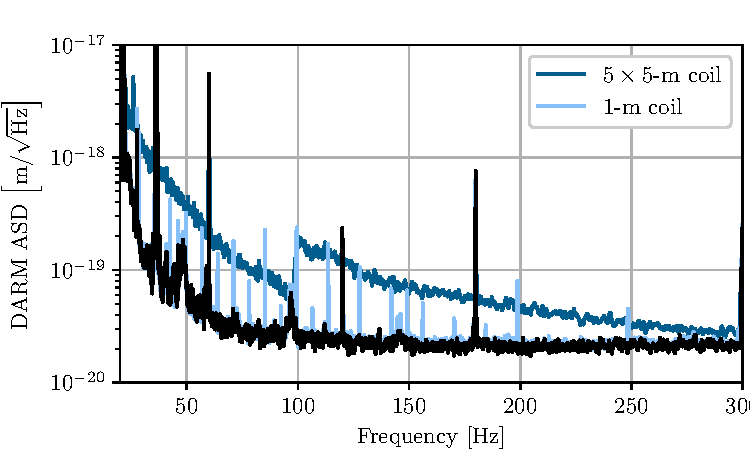
\includegraphics{figures/noise-methods/injection-wallcoil.pdf}
	\caption{
		Comparison of the old small-coil comb magnetic field injections with the new large-coil broadband injections.}
	\label{fig:injection-wallcoil}
\end{figure}

To achieve high-amplitude broadband magnetic injections, seven wall-mounted coils, each one a 3\,m x 3\,m or 5\,m x 5\,m square of 80-100\,turns, are being installed at each site; three at the corner station and two at each end station. These coils are fixed in place and can be operated remotely, allowing for weekly injections to monitor variations in magnetic coupling caused by changes to electronics. Figure~\ref{fig:injection-wallcoil} compares the old and new magnetic injections. Some coils were installed and operated at the sites during O3 (discussed in Section~\ref{sec:mag-weekly}); the project will be completed by the start of O4.




%%%%%%%%%%%%%%%%%%%%%%%%%%%%%%%%%%%%%%%%%%%%%%%%%%%%%%%%%%%%%%%%%%%%%%%%%%%%%%%%
%%% COUPLING FUNCTIONS %%%
%%%%%%%%%%%%%%%%%%%%%%%%%%%%%%%%%%%%%%%%%%%%%%%%%%%%%%%%%%%%%%%%%%%%%%%%%%%%%%%%



\section{Coupling functions}\label{sec:cf}

{\color{red}
Goal here is to give much more mathematical rigor to coupling function model than was provided in the relatively terse CF section of the PEM paper.
Still trying different notation conventions.
Hard to choose a convention for the many variables and indices that isn't confusing, since there are many similar but not identical quantities.}

\subsection{Single coupling site, sensor, and injection}

Suppose there exists exactly one coupling site, i.e. one location at which incident environmental signals result in excess noise in the \ac{GW} strain data.
Suppose also that a sensor is placed at the location of the coupling site, and a noise injection is performed that produces a signal observable by the sensor and the interferometer readout.
The coupling mechanism can be modeled in the frequency domain as a linear system:

\begin{equation}\label{eq:cf_model}
	h(f) = C(f) x(f),
\end{equation}
where $h(f)$ is the \ac{ASD} of the detector (strain) response, $x$ is the \ac{ASD} of the injection signal as measured by the sensor, and $C(f)$ is the \textit{coupling function}, which represents the amplitude of gravitational wave strain noise per unit amplitude in the sensor.
By convention, the strain is typically converted to \ac{DARM}, in meters, in which case $C(f)$ represents  test mass displacement per unit of sensor amplitude.
If the injection signal is an acoustic signal and the sensor is a microphone measuring amplitude in Pa, for instance, then the acoustic coupling function is in units of m/Pa.

In both the witness sensor and the detector, some ambient background noise is always present whether or not an injection is produced. Let $h\bkg(f)$ and $h\inj(f)$ be the \acp{ASD} of the detector during a period of background noise and during the injection, respectively. Likewise let $x\bkg(f)$ and $h\inj(f)$ be the background and injection \acp{ASD} of the sensor. Since the noise adds linearly in the power spectral domain, the actual signal in each is the difference between the injection-time and background-time \acp{PSD}:

\begin{align}
	\left[h(f)\right]^2 &= \left[h\bkg(f)\right]^2 - \left[h\bkg(f)\right]^2 \label{eq:h_inj}\\
	\left[x(f)\right]^2 &= \left[x\bkg(f)\right]^2 - \left[x\bkg(f)\right]^2 \label{eq:x_inj}
\end{align}

Combining~\crefrange{eq:cf_model}{eq:x_inj}, we can measure the coupling function from the background and injection \acp{ASD}~\citep{Kruk_2016, pem_code}:

\begin{equation}\label{eq:cf}
	\mathrm{C}(f) = \sqrt{\frac{[h_{\textrm{inj}}(f)]^2 - [h_{\textrm{bkg}}(f)]^2}{[x_{\textrm{inj}}(f)]^2 - [x_{\textrm{bkg}}(f)]^2}}.
\end{equation}
The value of a coupling function at a single frequency bin is referred to as a \textit{coupling factor}.

\subsection{Multiple coupling sites, sensors, and injections}

Suppose now there are multiple coupling sites, and a sensor is placed at the location of each site.
The detector response to an environmental signal now becomes a linear combination of the sensor signals and their sensor-specific coupling functions:

\begin{equation}\label{eq:cf_model_expanded}
	h(f) = \sum_{j=1}^{m} \mathrm{C}_j(f) x_{j}(f),
\end{equation}
Solving for the coupling function now would require producing multiple injections instead of just one, resulting in a system of $n$ equations with $m$ unknown coupling functions, where $n$ and $m$ are the numbers of injections and sensors, respectively:

\begin{equation}\label{eq:cf_full}
	h_i(f) = \sum_{j=1}^{m} \mathrm{C}_j(f) x_{ij}(f).
\end{equation}
Here $h_i(f)$ is the detector response during injection $i$, $x_{ij}(f)$ is the amplitude measured by sensor $j$ during injection $i$, and $\mathrm{C}_j(f)$ is the coupling function of sensor $j$.
If $n = m$,~\cref{eq:cf_full} could be solved to determine the coupling functions of all sensors.

Thus far it has been assumed that the witness sensors are placed precisely at the locations of the coupling mechanisms, but such perfect placement is not realistically feasible given that there are an unknown number of coupling sites at unknown locations.
A sensor, even if it is near a coupling site, only measures the injection amplitude at its own location, not at the coupling location.
Therefore, when using real-world sensors,~\cref{eq:x_inj} is not exact, so~\cref{eq:cf} does not exactly describe the coupling at the coupling site.
Nevertheless, as explained above, sensors are distributed in order to maximize coverage of coupling sites and this has been sufficient for producing reliable coupling functions for all sensors, as discussed further in Section~\ref{sec:uncertainties}.
As seen in Figure~\ref{fig:cf-cartoon-simple}, the sensor coupling function $C_j(f)$ is a good approximation to the true coupling $C(f)$ if the injection distance from the sensor $r_{ij}$ is much greater than the distance between the coupling site and sensor.
This allows us to estimate excess noise in the \ac{GW} channel $h_i(f)$ without directly measuring the coupling actuation $A_i(f)$.

\begin{figure}[h]
	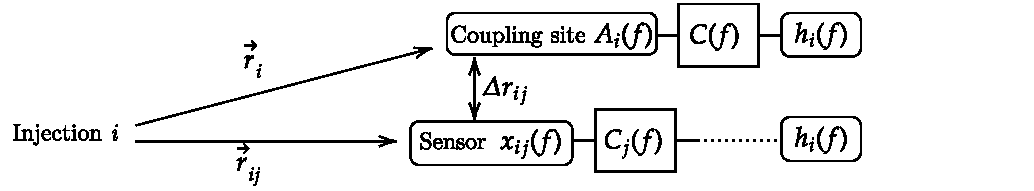
\includegraphics[width=\textwidth]{figures/noise-methods/cf-cartoon-simple.pdf}
	\caption
	[Diagram of a trivial coupling function measurement in the trivial case.]
	{
		Diagram of a coupling function measurement in the trivial case.
		An injection $i$ produces a signal $A_i(f)$ at a coupling site, which cannot be measured directly.
		If the injection is performed sufficiently far, then $\Delta r_{ij} \ll |\vec{r}_{ij}|$, so $C_j(f) \approx C(f)$.
	}
	\label{fig:cf-cartoon-simple}
\end{figure}

In Figure~\ref{fig:cf-cartoon-full} we can see how complex the experiment system becomes when there are multiple coupling sites of unknown location.
If there are two coupling sites $A$ and $B$, at least two injections $i_1$ and $i_2$ are required to distinguish between the coupling mechanisms.
The \ac{GW} channel response to injection $i_1$ is therefore the sum of the contributions of the actuation signals $A_{i_1}(f)$ and $B_{i_1}(f)$, and likewise for injection ${i_2}$.
Again, at best we merely approximate the actuations $A_i(f)$ and $B_i(f)$ with sufficiently close sensors, although we do not know \textit{a priori} which sensors are near coupling sites.

\begin{figure}[h]
	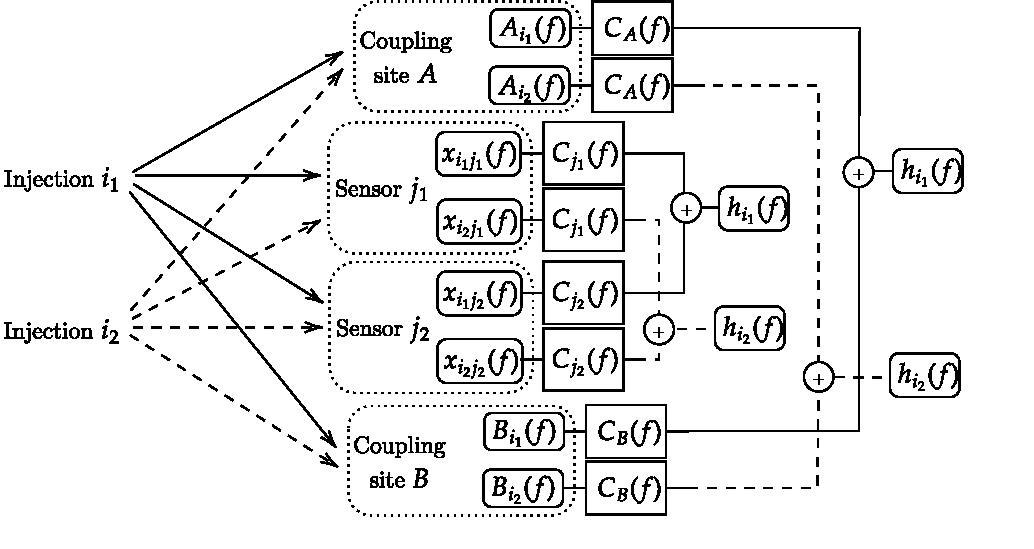
\includegraphics[width=\textwidth]{figures/noise-methods/cf-cartoon-full.pdf}
	\caption
	[Expanding Figure~\ref{fig:cf-cartoon-simple} to more than one sensor and coupling site.]
	{
		Expanding Figure~\ref{fig:cf-cartoon-simple} to two injections $i_1$ and $i_2$, two sensors $j_1$ and $j_2$, and two coupling sites $A$ and $B$.
		Each injection response $h_i(f)$ is itself a sum across contributions from $A$ and $B$.
		The goal is to determine the sensor couplings $C_j(f)$ that reproduce $h_i(f)$ using the sensor measurements $x_{ij}(f)$ since the true coupling actuations $A_i(f)$ and $B_i(f)$ are not known.
	}
	\label{fig:cf-cartoon-full}
\end{figure}

\subsection{Solving the coupling equations}

One hurdle remains in attempting to solve ~\cref{eq:cf_full}.
In practice, typically $n<m$ due to logistical constraints on the number of injections one could perform during a realistic time window, which makes the system of equations underdetermined.
A straight-forward least-squares regression is therefore not always feasible.
Below are two approximation methods for determining $C_j(f)$ for all sensors.

\textit{Nearest-sensors approximation}.
One method of forcing $n=m$ is reducing the number of sensors in each each equation, by asserting $x_{ij}(f)=0$ for sensors that are sufficiently far from the source of injection $i$.
This can be done by ordering the sensors by distance from the injection source and applying the assertion to the $m-n$ farthest sensors.
Issues can arise if there are sensors that are never near enough to any injection source, causing them to zeroed out for all injections; this requires that injections be distributed such that each sensor is near enough to at least one injection.

\textit{Nearest-injection approximation}.
Instead of solving \cref{eq:cf_full} in full, one can approximate $\mathrm{C}_j(f)$ for each sensor independently of other sensors.
Given a sensor $j$, \cref{eq:cf} can be repurposed by replacing $x$ with $x_{ij}$ and $h$ with $h_i$ to compute a single-injection ``coupling function'' $\mathcal{C}_{ij}(f)$ for each injection:

\begin{equation}\label{eq:sicf}
	\mathcal{C}_{ij}(f) = \sqrt{\frac{[h_{i,\textrm{inj}}(f)]^2 - [h_{i,\textrm{bkg}}(f)]^2}{[x_{ij,\textrm{inj}}(f)]^2 - [x_{ij,\textrm{bkg}}(f)]^2}}.
\end{equation}
The closer an injection is to a sensor $i$, the more accurately $\mathcal{C}_{ij}(f)$ approximates $\mathrm{C}_j(f)$, since the detector response would be dominated by coupling near sensor $j$.
Therefore one can construct the sensor coupling function by choosing at each frequency bin the coupling factor corresponding to the nearest injection, determined by the highest sensor amplitude (using the assumption that injection amplitudes are equivalent).
That is, for a frequency $f_k$ and a set of injections $\mathcal{I}$, one can measure the sensor amplitudes $\{x_{ij}(f_k)\ |\ i \in \mathcal{I}\}$, compute the single-injection coupling functions $\{\mathcal{C}_{ij}(f_k)\ |\ i \in \mathcal{I}\}$, and construct the approximate sensor coupling function

\begin{equation}\label{eq:ccf}
	\widetilde{\mathrm{C}}_j(f_k) := \mathcal{C}_{lj}(f_k)\ \mathrm{where}\ l = \mathop{argmax}_{i\in\mathcal{I}}\ (x_{ij}(f_k)).
\end{equation}
If the distribution of injection locations provides sufficient coverage of sensor locations, then $\widetilde{\mathrm{C}}_j(f) \approx \mathrm{C}_j(f)$.
Shortcomings of this assumption are discussed in Section~\ref{sec:uncertainties}.

Figure~\ref{fig:cf-example} provides an example of a single-injection coupling function measurement for a \ac{PSL} acoustic injection.
Figure~\ref{fig:cf-composite} shows an estimated ambient noise based on an accelerometer coupling function constructed from five single-injection coupling functions.
For simplicity only five injections were used to produce this example, however in practice the number of injections performed near a sensor can be much higher.

\begin{figure}
	\centering
	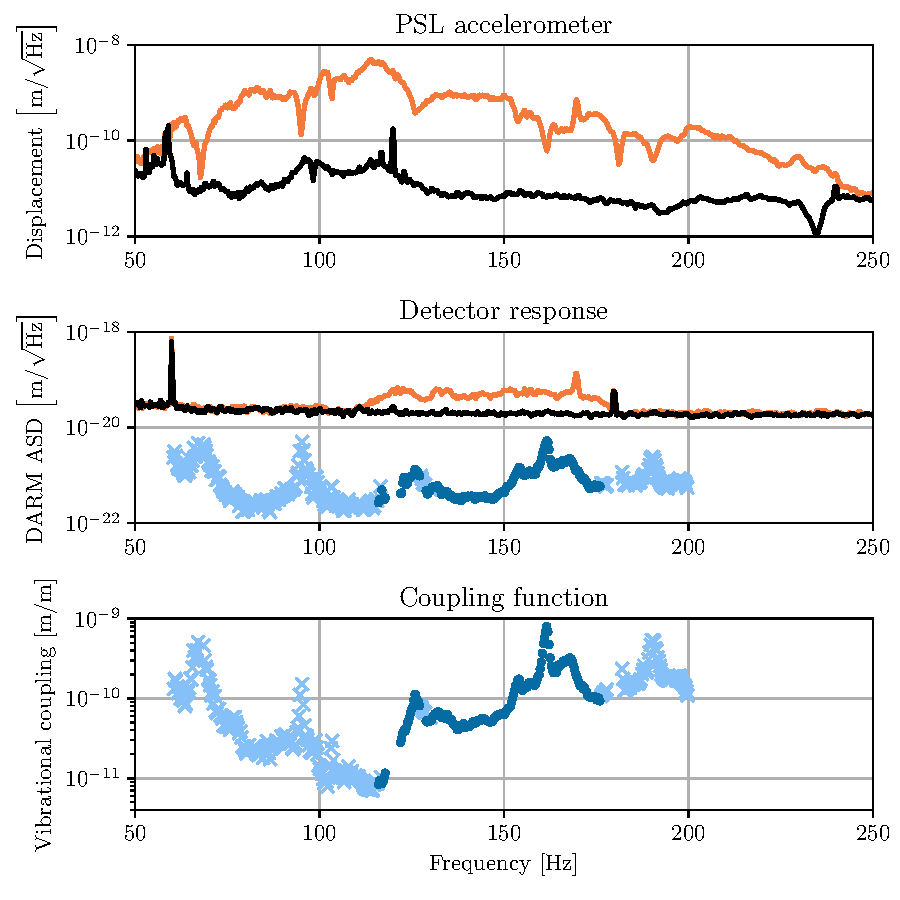
\includegraphics[width=\textwidth]{figures/noise-methods/cf-example.pdf}
	\caption
	[Example of a broadband acoustic noise injection and measurement of a single-injection coupling function]
	{
		Example of a broadband acoustic noise injection and measurement of a single-injection coupling function.
		Top: displacement of an accelerometer in the PSL room during background time (black) and injection time (orange).
		Middle: DARM during background time (black) and injection time (orange).
		Estimated ambient levels for the accelerometer are shown as dark blue dots, with upper limits shown as light blue crosses.
		Bottom: single-injection coupling function used to produce estimated ambient above.
		}
	\label{fig:cf-example}
\end{figure}

Due to hardware limitations it can be possible for an injection signal to be strong enough to produce excess noise in a sensor \ac{ASD} but not in the \ac{GW} detector \ac{ASD}.
For frequency bins where this is the case, an upper limit on $\mathcal{C}_{ij}(f_k)$ can be established by assuming, as a worst-case scenario, that all of the detector noise at that frequency is produced by the coupling alone

\begin{equation}\label{eq:siul}
	\mathcal{C}_{ij, \mathrm{UL}}(f) = \frac{h_{i,\textrm{bkg}}(f)}{\sqrt{[x_{ij,\textrm{inj}}(f)]^2 - [x_{ij,\textrm{bkg}}(f)]^2}}.
\end{equation}
The larger the injection amplitude, the better this upper limit can be constrained.
The boundaries between measurements, upper limits, and null results are established by two \ac{ASD} ratio thresholds: a sensor threshold and a detector threshold.
Let $r_x := x_{ij,\textrm{inj}}(f) / x_{ij,\textrm{bkg}}(f)$ and $r_h := h_{i,\textrm{inj}}(f) / h_{i,\textrm{bkg}}(f)$ represent the injection signal-to-noise ratios if the sensor and \ac{GW} detector \acp{ASD}, respectively.
If $r_x \geq t_x$ and $r_h \geq t_h$, where $t_x$ is the sensor threshold and $t_h$ is the detector threshold, then a measurement is computed via \cref{eq:sicf}.
Otherwise, if $r_x \geq t_x$ but $r_h < t_h$, then \cref{eq:siul} is used to place an upper limit on the coupling.
If $r_x < t_x$ and $r_h < t_h$, then neither a measurement nor upper limit is computed.
The null hypothesis is thus assumed:

\begin{equation}\label{eq:sinull}
	\mathcal{C}_{ij, \mathrm{null}}(f) = \frac{h_{i,\textrm{bkg}}(f)}{x_{i,\textrm{bkg}}(f)}.
\end{equation}

The values of $t_x$ and $t_h$ are determined based on typical level of random fluctuations observed in the spectra, but often values of $t_x = 10$ and $t_h = 2$ are used for most types of sensors and injections.
The higher choice of $t_x$ is due to the environmental sensors being much more sensitive to random fluctuations in the ambient noise level than the interferometer is.

The coupling function as approximated in \cref{eq:ccf} is used for comparing coupling between different sensor locations and producing estimates of interferometer noise levels, e.g. as part of event validation (see Section~\ref{sec:vetting}).
References to a sensor's coupling function will hereafter refer to this approximate quantity.
Figure~\ref{fig:cf-composite} provides an example of an estimated ambient for an accelerometer on the HAM6 vacuum chamber (which houses the interferometer output optics).
The \ac{PEM} website provides coupling functions for all accelerometers, microphones, and magnetometers produced from the most recent campaign of injections~\citep{PEM_website}.

\begin{figure}[h!]
	\centering
	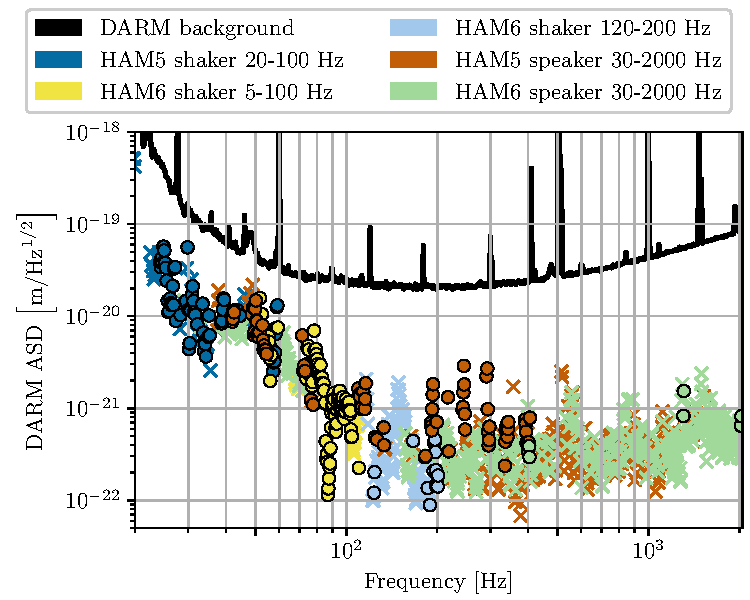
\includegraphics{figures/noise-methods/cf-composite.pdf}
	\caption
	[Ambient noise level for the LHO HAM6 Y-axis accelerometer]
	{
		Ambient noise level for the LHO HAM6 Y-axis accelerometer estimated from a composite coupling function, using acoustic and seismic injections near the output arm.
		}
	\label{fig:cf-composite}
\end{figure}

\section{Uncertainties and limitations of coupling functions}\label{sec:uncertainties}

\subsection{Comparison to transfer functions}

Environmental coupling is characterized using coupling functions instead of transfer functions because perfect coherence is not assumed in the system.
Low coherence can arise either due to non-linearity in the coupling or due to the spacing between the sensor and coupling site.
On a superficial level, a coupling function lacks a phase response component, representing only the magnitude response in the system.
Coupling functions also differ fundamentally from transfer functions in the sense that they do not assume the input signal to be the true actuation signal, but rather merely a witness of the actuation, while the actuation is in fact occurring at the location of the true coupling site.

\subsection{Assumptions about coupling mechanisms}

~\Cref{eq:cf} relies on two assumptions about the coupling mechanism.
First, the coupling is assumed to be linear in amplitude, e.g. doubling the amplitude of the injection would double the amplitude of the \ac{GW} detector response.
This is confirmed when performing injections by repeating them with different amplitudes and ensuring that the detector response scales proportionally with the injection amplitude.
Second, the coupling function ignores any up- or down-conversion of the signal between the sensor and the \ac{GW} detector.
Such non-linear coupling can be very significant for scattering noise and bilinear coupling, but is not accounted for in the estimates of linear coupling.
One way to check for non-linear coupling is by sweeping single frequency injections over time and searching for off-frequency responses in the \ac{GW} detector.
Frequency changes from non-linear coupling can be an issue in broadband injections where up- or down-converted noise in the interferometer readout appears in the injection band, resulting in artificially higher estimates at those frequencies.
We split broadband injections into smaller frequency bands to avoid this effect when necessary.
One approach for quantifying non-linear coupling is presented in \citet{Washimi_2020}.

\subsection{Hardware limitations}\label{sec:uncertainties-hardware}

\textit{Injection amplitudes}. To measure coupling, we inject signals large enough to produce a response in the detector, but the maximum amplitude of injections is limited by the sensitive range of the environmental sensors (saturation produces an overestimate of coupling).
This effectively limits how far below the detector noise background we can probe for coupling or establish upper limits.

Recall that \cref{eq:ccf} was based on assuming that injection amplitudes are equivalent.
However, this assumption is ambitious: since injections vary with distance to sensors, the amplitudes used have to be adjusted to achieve a large signals in the sensors and in the \ac{GW} channel.
This means that the highest-amplitude injection measured by a sensor is not necessarily the nearest injection to that sensor.
If a further injection was performed using a much larger amplitude, its measured amplitude can trump that of a nearer injection, leading to the algorithm choose a more distant injection source location when determining $\widetilde{\mathrm{C}}_j$.
To prevent this issue, once $\mathcal{C}_{ij}$ is computed for all sensors for a single injection, an additional sensor threshold is applied that is a fraction of the highest amplitude observed by all sensors.
This threshold is used only to demote measurements to upper limits.
By doing so, this injection-dependent threshold vetos measurements produced by sensors that are far from the injection.
For the \ac{O3} injections, the threshold was set at one third, meaning that a coupling measurement is demoted to an upper limit if the sensor measuring it observes the injection at less than a third of the amplitude observed by the sensor closest to the injection.

{\color{red}
Need to talk about this a lot more.
Injection-depended thresholding reflects a fundamental issue with the distribution of sensors and injections.
In principle if you have many one-to-one correspondence b/w sensors and injections,
you would just have each injection produce measurements in its nearest sensor, which is effectively what you get by setting this threshold to one.
But in absence of that ideal injection distribution you have to lower the threshold by some amount and it's not obvious how to operationalize this.
Nevertheless some even as an ad hoc thresholding scheme it works very well for preventing inaccurate coupling functions from misattributing the nearest injection to a sensor.

I need to emphasize that this is basically a way of normalizing injections.}

\textit{Uncertainty due to injection locations}.
As mentioned above, the model in \cref{eq:cf_full} relies on the assumption that the environment is monitored at the coupling site.
The density of sensors is not great enough for this to be strictly true, especially if the source of the environmental signal is closer to the coupling site than the sensor is.
The detector response to an injection depends on the distance between the injection and coupling site, whereas the sensor response depends on the distance between the injection and sensor.
Varying the injection location therefore varies the relative scaling of the numerator and denominator of \cref{eq:sicf}, affecting the measurement of $\mathcal{C}_{ij}(f)$ and subsequently the sensor coupling function via \cref{eq:ccf}.
Therefore, a finite spacing of sensors leads to some degree of uncertainty in the coupling functions.
This uncertainty also propagates to projected noise levels in the \ac{GW} channel using these coupling functions.

\begin{figure}[h!]
	\centering
	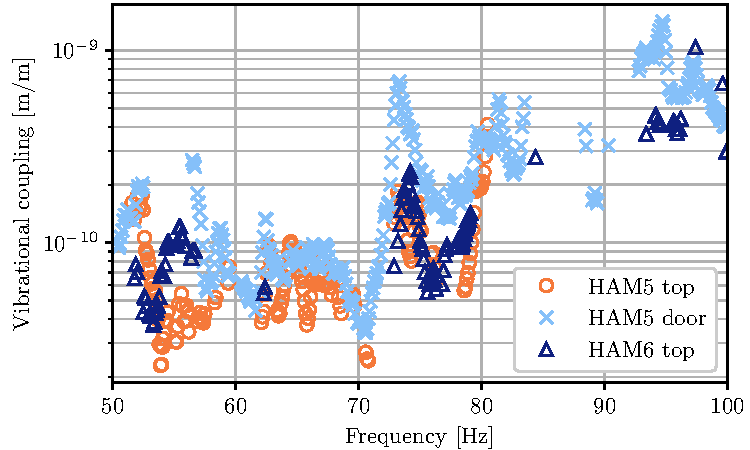
\includegraphics[width=\textwidth]{figures/noise-methods/cf-locations-vib.pdf}
	\caption{
		Single-injection coupling functions (upper limits not shown) for the HAM5 Y-axis accelerometer for three different shaker injection locations (on top of HAM5, on top of HAM6, and on the HAM5 chamber door).}
	\label{fig:cf-locations-vib}
\end{figure}

Since the uncertainty manifests as a multiplicative scaling of $\mathcal{C}_{ij}(f)$, it can be described by computing a geometric standard deviation of $\mathcal{C}_{ij}(f)$ for a single sensor over a range of injection locations, at each frequency bin.
Figure~\ref{fig:cf-locations-vib} shows single-injection coupling functions for an accelerometer measured from shaker injections produced from three locations (the distribution of injection locations is discussed in Section~\ref{sec:injections}.
Since the injection locations are close enough to the accelerometer, it can be assumed that the variance is primarily due to finite spacing effect.
Averaged across all frequency bins, the geometric standard deviation between injection locations is 1.4, i.e. coupling functions measured from vibrational injections can be expected to vary by a factor of 1.4 when measured by different injection locations.

\begin{figure}[h!]
	\centering
%	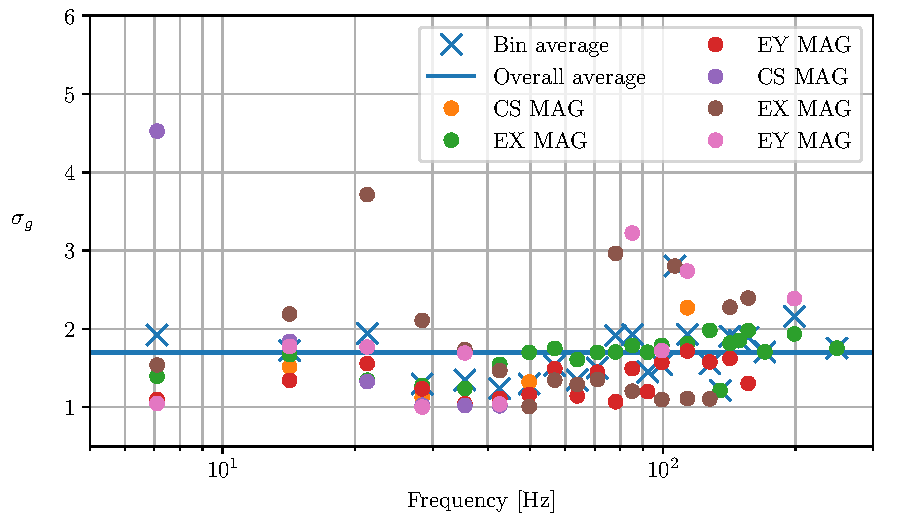
\includegraphics[width=\textwidth]{figures/noise-methods/cf-locations-mag.pdf}
	\caption{
		Single-injection coupling functions (upper limits not shown) for various magnetometers and various injections at both observatories.}
	\label{fig:cf-locations-mag}
\end{figure}

A similar study was performed combining geometric standard deviations for various magnetometers at both observatories.
There are fewer magnetic injection locations to use for the comparison, but since coupling can be measured at each station (a corner station and both end stations) at each of the two LIGO observatories, there are twelve magnetometers that can be used, each with two or more injections nearby.
The result of this study is that magnetic coupling measurements and noise projections vary by a factor of 1.7.
This is slightly greater than that of vibrational measurements, since the lower number of magnetometers means that the distances between coupling sites and sensors is greater, amplifying the finite spacing effect.

For both vibrational and magnetic coupling, these estimated uncertainties are acceptable given that conclusions made from coupling functions are often more qualitative than strictly quantitative, i.e. identifying and localizing coupling mechanisms is more important that precise estimates of the detector response.
That said, more precise noise estimates may become important for quantifying the impact of environmental transients on \ac{GW} event candidates, as discussed in Section~\ref{sec:vetting}.

\textit{Nodal artifacts from acoustic injections}.
In the case of acoustic injections, the uncertainty in a coupling function can be exacerbated when nodes and anti-nodes in the acoustic signal coincide with the location of a sensor but not a coupling site.
This results in peaks and troughs in the sensor spectrum at frequencies that have a node or anti-node at the sensor location, respectively.
These artifacts can impact any sensor, but are more noticeable in microphone spectra than accelerometer spectra, possibly because the stiffness of the vacuum enclosure results in effectively averaging over a larger area; in microphones, the peak-to-trough ratio is typically a factor of a few.
The peaks and troughs are present in the sensor but not in the detector spectrum, because the sensor monitors a single point whereas the coupling to the interferometer is spread across a large enough area for the effects of nodes and anti-nodes to average out.
Consequently, this effect imprints troughs and peaks onto the coupling function.

The artifacts can be smoothed out of the spectra by applying a moving average over $x_{ij,\mathrm{inj}}(f)$ before computing $\mathcal{C}_{ij}(f)$.
The moving average window must be on the scale of a few Hz since this is typically the scale of the peak-to-peak distances.
On the other hand, smoothing of spectra can also result in less accurate coupling measurements when narrow mechanical resonances are present, so the window must balance the smoothing of artifacts against this disadvantage.
For accelerometer spectra, analyzing injections with various smoothing parameters show that a logarithmically-scaled window which is \XX\,Hz wide at 100\,Hz and \XX\,Hz wide at 1000\,Hz best satisfy these constraints.
Since microphones are much more sensitive to nodal artifacts while being less sensitive to narrow mechanical resonances (they would have to be strong enough to produce audible signals), their spectra can be smoothed much more aggressively: a logarithmically-scaled window is used which is 15\,Hz wide at 100\,Hz and 150\,Hz wide at 1000\,Hz.

\section{The {\fontfamily{pcr}\selectfont pemcoupling}\xspace package}
\label{sec:pemcoupling}

This section covers the technical details of the \pemcoupling python package~\citep{pem_code}, which includes command-line tools for processing large numbers of injections and producing single-injection coupling functions, coupling functions, and multi-channel summary coupling functions.

The package uses the \code{gwpy} library for fetching raw time series data and producing \acp{ASD} of the \ac{GW} strain channel and auxiliary channels from user-provided background and injection times.

\subsection{Processing steps}

{\color{red}
This subsection is quite messy.
The confusion comes from talking about different sensors at different steps.
I think I could try splitting it by sensor type, like list all steps for accelerometers and microphones, then all steps for magnetometers.}

A number of pre-processing steps are performed to condition the data for analysis.
First, the auxiliary channel time series are examined for evidence of saturation.
Injections can cause saturation in two ways: actuator saturation due to overdriven amplifiers, or sensor saturation due to hitting the maximum amplitude the sensor can record.

During magnetic injections, the injection amplitude typically has to exceed background by a few orders of magnitude to produce noise in the \ac{GW} channel, so comb magnetic injections are the most likely to saturate at the actuator.
They are also capable of saturating the sensors if performed too close (such as in the electronics racks).
In either case, intermodulation distortion occurs, generating peaks at sums and differences of the comb line frequencies while also reducing signal power in the injection lines.
If the saturation is occuring at the actuator, the measured coupling is still accurate, but upper limits are higher due to the reduced signal power.
On the other hand, sensor saturation results in inaccurate coupling measurements, because the line amplitudes no longer reflect the true magnetic signal at the sensor location.

Accelerometers can saturate in the presence of broadband vibrational injections.
This results in artificial broadband noise in the amplitude spectra.
The consequence is measuring a lower coupling function at frequencies where the saturation artifact dominates.

For these reasons, coupling functions are only measured for sensors that do not exceed 32,000 counts, as this is the sign of sensor saturation.

Once the time series are converted to \acp{ASD}, tri-axial magnetometer channels are combined in quadrature.
Each magnetometer measures the $x$, $y$, and $z$ components of its local magnetic field independently.
An artificial channel is produced to represent the absolute magnitude of the field.

All \ac{PEM} channels have accompanying calibration measurements~\citep{PEM_website}. Calibration for microphones and magnetometers is simply a constant conversion of Pa/count or T/count, respecitvely.
Accelerometer \acp{ASD} are converted to acceleration ($\mathrm{m/s^2}$), then to displacement ($\meter$) by dividing each bin by $(2\pi f)^2$ where $f$ is the bin frequency.

For acoustic injections, spectral smoothing is applied at this point, in order to surpress nodal artifacts as explained in Section~\ref{sec:uncertainties-hardware}.
Finally, the single-injection coupling funcitons $\mathcal{C}_{ij}(f)$ and upper limits $\mathcal{C}_{ul}(f)$ are measured as in~\cref{eq:sicf}.

{\color{red}
Paragraph or two on the CF calculation step.}

\subsection{Data products}

For each $\mathcal{C}_{ij}(f)$, the data are saved in the following forms:
\begin{enumerate}
	\item comma-separated text file consisting of coupling measurements, flags, and raw spectra
	\item plot of the  raw coupling function (units of meters per analog-to-digital counts)
	\item plot of the coupling function in physical units (meters per calibrated sensor unit, e.g. Tesla for magnetometers)
	\item figure containing two subplots: one showing the background and injection spectra of the auxiliary sensor, and one showing the background and injection spectra of the \ac{GW} strain data and the estimated environmental noise projection.
\end{enumerate}

\begin{table}\label{tab:pemcoupling-format}
	\renewcommand{\arraystretch}{1.5}
	\begin{tabular}{|ll|}
		\hline
		\multicolumn{1}{|l}{\textbf{column}} & \multicolumn{1}{l|}{\textbf{description}}\\ \hline
		\code{frequency}      & bin center frequency {[}Hz{]}\\
		\code{factor}         & coupling factor in {[}m/calibrated sensor unit{]}\\
		\code{factor\_counts} & coupling factor in {[}m/ADC count{]}\\
		\code{flag}           & ``Measured", ``Upper Limit", ``Thresholds not met", or ``No data"\\
		\code{sensINJ}        & sensor amplitude at injection time {[}calibrated sensor unit$/\rthz${]}\\
		\code{sensBG}         & sensor amplitude at background time {[}calibrated sensor unit$/\rthz${]}\\
		\code{darmINJ}        & \ac{GW} channel amplitude at injection time $[\meter/\rthz]$\\
		\code{darmBG}         & \ac{GW} channel amplitude at background time $[\meter/\rthz]$\\ \hline
	\end{tabular}
	\caption{Column descriptions for the single-injection coupling function output of the \pemcoupling package.}
\end{table}

Post-processing, to aggregate single-injection coupling functions into coupling functions, and produce site-wide coupling plots, is done via additional commands, \code{pemcoupling-composite} and \code{pemcoupling-summary}.

{\color{red}
Expand on these final steps a bit.}
